\appendix

\section{Full Pruning Results}
\label{app:full_results}

Table~\ref{tab:full_results} reports the complete closed-loop success rates for all four models across all tested retention ratios, including OpenVLA and $k{=}0.7$ data omitted from Table~\ref{tab:main_results} for space.

\begin{table*}[ht]
\centering
\footnotesize
\caption{Available closed-loop success rates (\%) on LIBERO under L2 norm (L2) and random (R) token pruning. Best result per row in \textbf{bold}. ``--'' indicates condition not evaluated. OpenVLA Goal, Spatial, and Long use per-suite fine-tuned checkpoints. Single seed (seed 42) except $\pi_{0.5}$ Long (five-seed mean, $n{=}5$). \textsuperscript{$\dagger$}Attention-based scoring (A) at $k{=}0.9$ for OpenVLA.}
\label{tab:full_results}
\setlength{\tabcolsep}{4pt}
\begin{tabular}{llccccc}
\toprule
Model & Suite & Baseline & $k{=}0.95$ (L2 / R) & $k{=}0.9$ (L2 / R) & $k{=}0.7$ (L2 / R) & $k{=}0.5$ (L2 / R) \\
\midrule
\multirow{4}{*}{$\pi_{0.5}$}
& Object  & \textbf{98.2} & 98.2 / 74.0 & \textbf{98.2} / 9.0 & 55.0 / 74.0 & 33.4 / 69.4 \\
& Spatial & \textbf{97.2} & \textbf{97.8} / 76.4 & 95.0 / 54.6 & 67.0 / 74.4 & 55.6 / 71.6 \\
& Goal    & \textbf{96.4} & 89.4 / 84.0 & 90.6 / 62.2 & 71.2 / 78.2 & 59.2 / 73.6 \\
& Long    & \textbf{91.6} & 86.8 / 61.2 & 80.4 / 33.6 & 63.2 / 64.6 & 51.7 / 50.4 \\
\midrule
\multirow{4}{*}{X-VLA}
& Object  & \textbf{99.2} & 99.0 / 98.8 & 99.2 / 97.8 & 56.2 / 65.2 & 43.4 / 70.6 \\
& Spatial & \textbf{93.0} & 71.6 / 70.2 & 78.8 / 77.8 & 72.0 / -- & 58.8 / 71.4 \\
& Goal    & \textbf{98.4} & 53.8 / 54.0 & 70.2 / 70.6 & 53.4 / 57.2 & 59.0 / 67.2 \\
& Long    & \textbf{94.0} & 47.0 / 48.2 & 27.5 / 29.6 & -- / -- & 45.0 / 61.6 \\
\midrule
\multirow{4}{*}{OpenVLA}
& Object  & \textbf{74.0} & 70.6 / -- & 70.6 / 62.8 / 61.4\textsuperscript{$\dagger$} & -- / -- & 39.2 / 35.8 \\
& Goal    & \textbf{74.8} & -- / -- & 74.8 / 79.6 / 73.2\textsuperscript{$\dagger$} & -- / -- & -- / -- \\
& Spatial & \textbf{80.0} & -- / -- & 75.0 / 79.8 / 80.4\textsuperscript{$\dagger$} & -- / -- & -- / -- \\
& Long    & \textbf{52.8} & -- / -- & 43.6 / 46.8 / 44.0\textsuperscript{$\dagger$} & -- / -- & -- / -- \\
\midrule
\multirow{4}{*}{SmolVLA}
& Object  & \textbf{59.2} & 0.0 / 0.0 & 0.0 / 0.0 & 0.0 / 0.0 & 0.0 / 0.0 \\
& Spatial & \textbf{44.6} & 6.6 / 4.2 & 0.0 / 0.0 & 0.0 / 0.0 & 0.0 / 0.0 \\
& Goal    & \textbf{60.8} & 3.4 / 4.2 & 0.0 / 0.0 & 0.0 / 0.0 & 0.0 / 0.0 \\
& Long    & \textbf{36.6} & 0.0 / 0.0 & 0.0 / 0.0 & 0.0 / 0.0 & 0.0 / 0.0 \\
\bottomrule
\end{tabular}
\end{table*}


\section{Extended Discussion}
\label{app:extended_discussion}
\label{app:discussion}

\paragraph{Re-encoding and CV diagnostics.}
Both cross-attention and MLP modules achieve comparable recovery ($p = 0.15$); the stable M-curve ($M{=}16 \approx M{=}128$) confirms token count is secondary once entanglement is broken (Appendix~\ref{app:reencoding_analysis}). CV captures effective pipeline complexity beyond connector labels, differentiating X-VLA's threshold-graded behavior (CV$\,{=}\,$0.151) from $\pi_0$'s uniformly critical profile (CV$\,{=}\,$0.038); the interaction reverses at $k{=}0.3$ (Appendices~\ref{app:cv_strategy_interaction},~\ref{app:cv_extended}).

\paragraph{Task complexity compresses the importance margin.}
CV predicts connector-level compressibility, but task complexity determines \emph{which} scoring method succeeds within a given connector. OpenVLA illustrates the full pattern across LIBERO's complexity gradient (Figure~\ref{fig:openvla_sweep}).

On single-step Object, L2 leads at moderate pruning ($+$7.8\,pp at $k{=}0.9$), but the three methods exhibit staggered cliffs (L2 earliest ($k{=}0.9{\to}0.85$, $-$15.4\,pp), random next, attention latest), each defining a distinct effective compression window before converging at $k{=}0.5$ ($<$4.8\,pp spread). As task complexity increases, the scoring hierarchy inverts. On Goal, random pruning at $k{=}0.9$ \emph{exceeds} the unpruned baseline ($+$4.8\,pp; cross-seed confirmed), suggesting OpenVLA's 256 vision tokens are over-provisioned for goal-conditioned tasks; random removal acts as implicit regularization. On Long, the inversion is complete: at $k{=}0.7$, Random (38.8\%) $>$ L2 (31.2\%) $>$ Attention (24.0\%), with attention degrading $2.5{\times}$ faster than random. The mechanism is consistent: multi-step tasks distribute critical information across tokens with heterogeneous norm profiles; L2 and attention both cluster on locally salient tokens, sacrificing the spatial diversity that compositional reasoning requires.

\begin{figure}[ht]
\centering
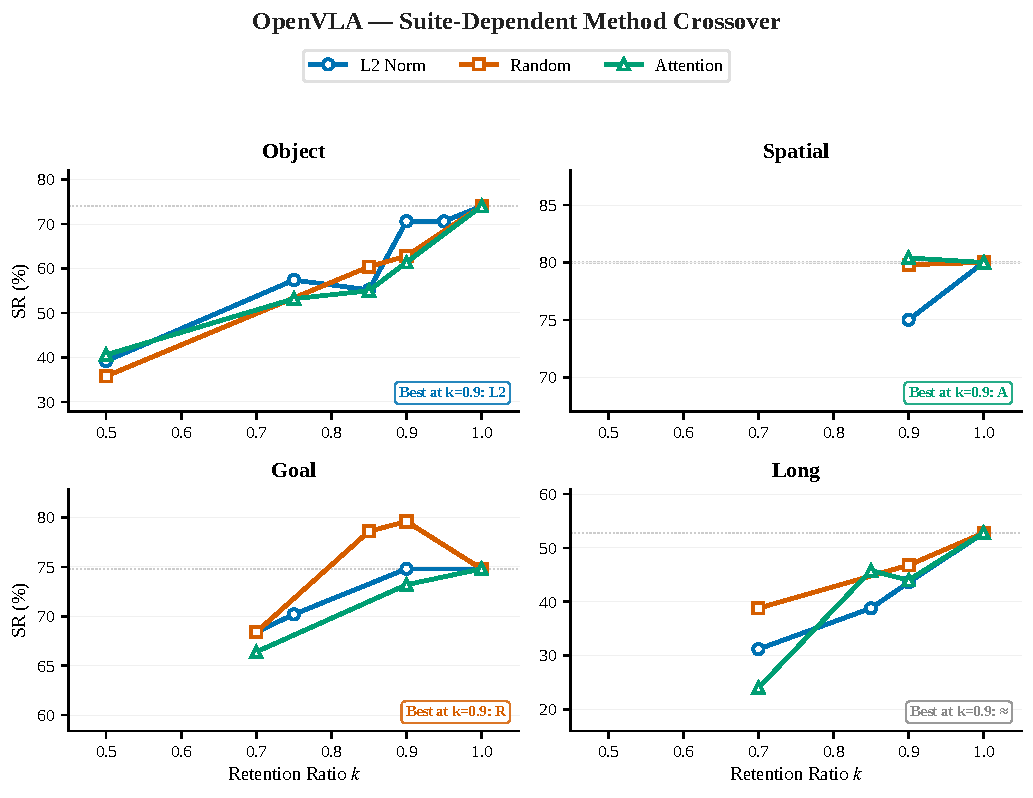
\includegraphics[width=\linewidth]{figures/paper/fig_openvla_sweep.pdf}
\caption{OpenVLA scoring method comparison across four LIBERO suites. On Object, L2 leads at $k{=}0.9$ ($+$7.8\,pp) but the margin flips at $k{=}0.85$ ($-$5.2\,pp, Random wins). Goal degrades smoothly with three-method convergence at $k{=}0.7$. On Long, the ranking inverts with compression. No single scoring method dominates across suites or retention ratios.}
\label{fig:openvla_sweep}
\end{figure}

This is a concrete manifestation of the two-axis framework (Section~\ref{sec:two_axis}): Axis~1 (connector architecture) determines \emph{whether} pruning is viable; Axis~2 (task complexity) determines \emph{which} scoring method succeeds. CV remains a valid connector diagnostic, but the optimal scoring strategy requires knowledge of both axes.

\paragraph{Position encoding mediates the V-shape recovery.}
The monotonic L2 curve versus the non-monotonic random curve on $\pi_{0.5}$ Long (Figure~\ref{fig:cliff_highlight}) reflects an interaction between token selection strategy and positional encoding. L2 norm scoring preserves spatial locality: retained tokens form near-contiguous clusters in the ViT grid, producing continuous position shifts after re-indexing that Gemma's RoPE accommodates smoothly, producing monotonic degradation (86.8\% $\to$ 51.7\% from $k{=}0.95$ to $k{=}0.5$). Random selection creates scattered gaps that produce position aliasing after re-indexing. At $k{\approx}0.9$, the aliasing is maximally destructive: a small number of randomly placed gaps create highly irregular inter-token spacing, collapsing SR to 33.6\%. Per-task analysis reveals this aggregate is driven by specific tasks with position-sensitive spatial reasoning: Task~4 (``put mugs on plates'') drops from 80\% at $k{=}0.7$ to 12\% at $k{=}0.85$, contributing disproportionately to the V-shape minimum. At $k{=}0.7$, enough tokens are removed that the surviving positions become approximately uniform again, and SR recovers to 64.6\%, exceeding the $k{=}0.9$ level by ${\sim}2{\times}$. The zero-mask ablation (Section~\ref{sec:zeromask}) provides causal confirmation: zeroing token content while preserving positions yields 98.0\% SR, while physically removing the same tokens collapses to 9.0\%. Position encoding, not information content, is the binding constraint, and scoring method determines whether that constraint is violated.

\paragraph{Per-task reversal within L2-dominant regimes.} The Long $k{=}0.85$ aggregate ($+$33.2\,pp for L2) masks extreme per-task heterogeneity (per-task $\sigma{=}$21.5\,pp). L2 outperforms random on 9 of 10 tasks ($+$16 to $+$52\,pp), but on Task~6, a dual-object spatial-relation task (``place white mug on plate \emph{and} chocolate pudding to the right of plate''), L2 collapses to 8\% while random achieves 52\% ($-$44\,pp reversal). L2 scoring systematically undervalues tokens encoding spatial relationships, which carry low norms but are critical for relational reasoning. This per-task sign flip within an architecture where L2 dominates overall reinforces that no single scoring method is universally safe: task semantics, not just connector architecture or suite-level statistics, determine optimal strategy.

\begin{figure}[ht]
\centering
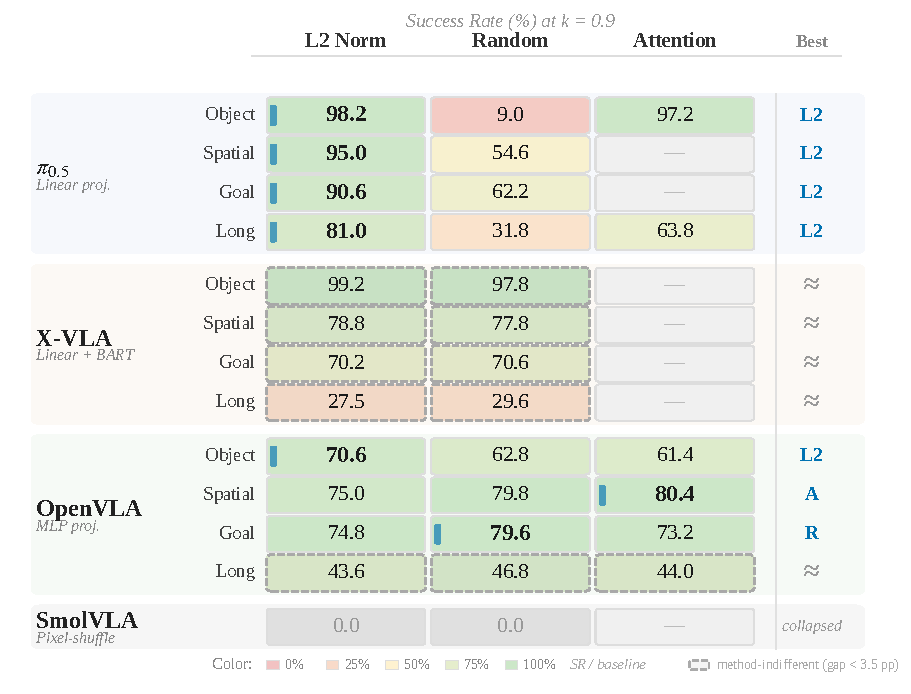
\includegraphics[width=0.85\linewidth]{figures/paper/fig_scoring_crossover.pdf}
\caption{Scoring method comparison at $k{=}0.9$ across three models and four LIBERO suites. Cell color encodes SR as a fraction of unpruned baseline; blue bars mark the best method per condition; dashed borders indicate method-indifferent cells ($\Delta{<}3.5$\,pp). $\pi_{0.5}$'s linear connector strongly favors L2 selection, while X-VLA's BART encoder is largely method-indifferent. SmolVLA collapses to 0\% regardless of method. Compact 2$\times$2 summary in Appendix Table~\ref{tab:scoring_crossover_summary}.}
\label{fig:scoring_crossover}
\end{figure}

\begin{figure}[ht]
\centering
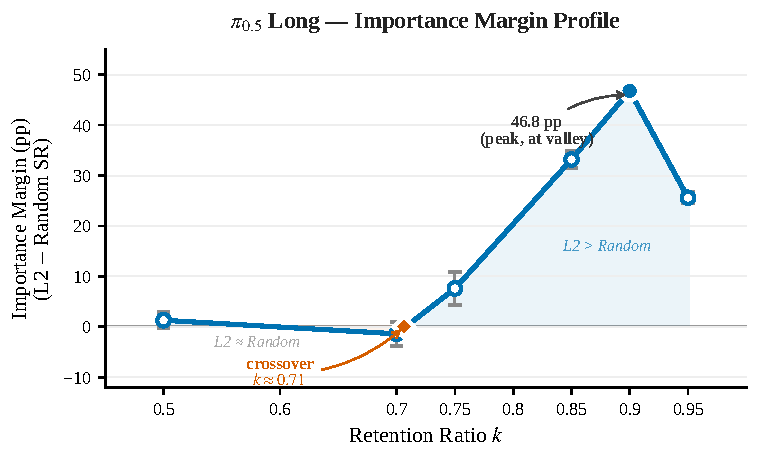
\includegraphics[width=0.85\linewidth]{figures/paper/fig_margin_profile.pdf}
\caption{Importance margin (L2 $-$ Random SR) on $\pi_{0.5}$ Long across retention ratios (multi-seed mean $\pm$ s.d.; $n{=}5$). The margin peaks sharply at $k{=}0.9$ (46.8\,pp) where random pruning is maximally destructive, then declines asymmetrically: one step above the peak ($k{=}0.95$: 25.6\,pp) versus four steps below before crossing zero at $k{\approx}0.71$. At $k{=}0.5$, L2 and Random converge ($|\Delta|{\approx}1.3$\,pp), indicating that scoring method choice matters only in the moderate-pruning window.}
\label{fig:margin_profile}
\end{figure}

\paragraph{Limitations (extended).}
All closed-loop evaluations use the LIBERO simulation benchmark; real-robot validation is absent. The six architectures differ in backbone capacity, vision encoder, and fusion strategy beyond the connector, so the connector effect cannot be causally isolated. $\pi_{0}$ and OFT are evaluated through offline metrics only, without closed-loop verification. The CV diagnostic spans six architectures across all three connector families; closed-loop validation covers four models ($\pi_{0.5}$, X-VLA, OpenVLA, SmolVLA). SmolVLA baselines (59.2\% official, 44.8\% LoRA reproduction) are substantially weaker than those of the other models; whether VTR recovery generalizes to stronger baselines is unknown.

\paragraph{Non-monotonicity as structural property.}
X-VLA on Goal exhibits non-monotonic degradation: $k{=}0.95$ drops to 53.8\% (L2) and 54.0\% (random), while $k{=}0.9$ recovers to 70.2\% under L2 selection (Table~\ref{tab:main_results}). The 0.2\,pp method gap at $k{=}0.95$ confirms that the anomaly is independent of the token scoring criterion. This pattern is consistent with position sensitivity in the 12-layer BART encoder~\cite{lewis2020bart}, where specific token positions carry disproportionate structural importance regardless of content.

\paragraph{$\pi_{0.5}$ random subsampling anomaly and RoPE amplification.}
Random selection on $\pi_{0.5}$ Object collapses from 74.0\% at $k{=}0.95$ to 9.0\% at $k{=}0.9$, then recovers to 74.0\% at $k{=}0.7$ (Table~\ref{tab:main_results}). The re-indexing step of our pruning protocol (Section~\ref{sec:pruning_protocol}) contributes to this non-monotonicity. $\pi_{0.5}$'s linear connector preserves a one-to-one mapping between spatial patches and token positions; when random removal shifts surviving tokens to new positions, the backbone's Rotary Position Embeddings (RoPE)~\cite{su2024roformer} encode spatial content at unfamiliar positions, amplifying disruption of learned attention patterns. X-VLA's BART encoder, which redistributes spatial information via cross-attention and lacks RoPE, provides a partial control. At $k{=}0.85$, single-step suites degrade smoothly (Spatial~68.2\%, Object~65.0\%, Goal~60.4\%), but Long drops to 35.0\%, below its $k{=}0.5$ performance of 61.6\% (Table~\ref{tab:xvla_k085_crosssuite}). Random re-indexing thus induces non-monotonic behavior for complex tasks even without RoPE, but RoPE amplifies the reversal: $\pi_{0.5}$ Object drops to 5.6\% at $k{=}0.85$ versus 69.4\% at $k{=}0.5$ ($-$63.8\,pp), more than double X-VLA Long's $-$26.6\,pp. The V-shaped recovery at $k \leq 0.7$ remains unexplained.

\begin{table}[ht]
\centering
\small
\caption{Random pruning at $k{=}0.85$: X-VLA (BART encoder) vs.\ $\pi_{0.5}$ (linear connector). X-VLA degrades smoothly on single-step suites (60--68\%) but drops to 35.0\% on Long (below $k{=}0.5$); $\pi_{0.5}$ exhibits a severe disruption peak on Object.}
\label{tab:xvla_k085_crosssuite}
\begin{tabular}{lcccc}
\toprule
Suite & X-VLA SR (\%) & $\Delta$ & $\pi_{0.5}$ SR (\%) & $\Delta$ \\
\midrule
Object & 65.0 & $-$34.2 & 3.6--5.6\textsuperscript{$\dagger$} & $-$93 to $-$95 \\
Goal & 60.4 & $-$38.0 & 52.4 & $-$44.0 \\
Spatial & 68.2 & $-$24.8 & --- & --- \\
Long & 35.0 & $-$59.0 & --- & --- \\
\bottomrule
\multicolumn{5}{l}{\footnotesize\textsuperscript{$\dagger$}Two seeds: seed42$\,{=}\,$5.6\% (post-fix), seed43$\,{=}\,$3.6\%. $\Delta$ from respective baselines.}
\end{tabular}
\end{table}

\paragraph{Small-$N$ interactions.}
X-VLA operates with only 50 vision tokens. At $k{=}0.95$, removing 3 tokens produces $-$44.6\,pp on Goal and $-$47.0\,pp on Long (L2 norm selection). Absolute token count interacts with CV: identical retention ratios impose qualitatively different damage when the token budget is small.

\paragraph{Design implications.}
Practitioners should compute importance CV before deploying token pruning, as low-CV and entangling-connector models require distinct compression strategies. Pixel-shuffle connectors need learned re-encoding rather than hard deletion. Task complexity must factor into pruning budget decisions: retention ratios safe for simple manipulation may fail on compositional tasks.


\section{Cross-Suite Task Complexity Analysis}
\label{app:cross_suite_extended}

LIBERO's four suites form a complexity gradient: Object and Spatial require single-step manipulation with explicit spatial cues, while Goal and Long demand multi-step planning, goal inference, or extended temporal coordination. This gradient interacts with pruning tolerance in a connector-dependent manner.

$\pi_{0.5}$ shows moderate complexity amplification under L2 norm pruning at $k{=}0.95$: Object retains 98.2\% (matching the baseline), Spatial retains 97.8\% (within noise of the 97.2\% baseline), and Goal drops to 89.4\% ($-$7.0\,pp from 96.4\%). Simple tasks absorb mild pruning with negligible loss; compositional tasks expose measurable degradation even at 5\% token removal.

X-VLA exhibits dramatic complexity amplification. At $k{=}0.9$ with L2 norm selection, Object retains 99.2\% (matching the 99.2\% baseline), while Goal drops to 70.2\% ($-$28.2\,pp from 98.4\% baseline). Under random pruning at the same ratio, Object loses just 1.4\,pp (97.8\%) while Goal loses 27.8\,pp (70.6\%), a $20{\times}$ amplification. The effect is even more pronounced at $k{=}0.95$ on Long: removing just 3 of 50 tokens collapses SR from 94.0\% to 47.0\% (L2) and 48.2\% (random), a 47.0\,pp loss with only 1.2\,pp method gap, while Object at the same ratio loses only 0.2\,pp.

Token-entangling connectors (X-VLA's BART encoder) amplify task complexity because compositional tasks require integrating information across spatial locations. When the BART encoder creates cross-token dependencies, removing even a few tokens disrupts the distributed representations that multi-step tasks rely on. Token-independent connectors ($\pi_{0.5}$'s linear projection, OpenVLA's MLP) show moderate complexity amplification because each token's contribution is self-contained: removing tokens reduces spatial coverage proportionally, and simple tasks tolerate the resulting gaps.


\section{Pruning Protocol Details}
\label{app:pruning_details}

Both pruning methods physically remove unselected tokens from the sequence, reducing the actual input length to the LLM rather than zeroing them out; zero-masking preserves positional structure while physical removal does not. After removal, remaining tokens retain their original spatial ordering; position IDs are re-indexed contiguously.

Model-specific retention ratios reflect each architecture's token count and expected sensitivity. $\pi_{0}$ is evaluated offline only ($k{=}0.1$, normalized L1 action loss; offline metrics only, no closed-loop evaluation available) because its deployment environment precludes closed-loop testing. $\pi_{0.5}$ uses $k \in \{0.3, 0.5, 0.7\}$ under both L2 and random removal; the dual-method design enables direct comparison within a single architecture. Pruning is applied per-image: each camera view independently retains the top-$k$ fraction. X-VLA spans $k \in \{0.1, 0.2, 0.3, 0.5, 0.7, 0.8, 0.85, 0.9, 0.95\}$ with L2 removal across three seeds, supplemented by random removal at selected $k$ values. OpenVLA uses $k \in \{0.3, 0.5, 0.7, 0.9, 0.95\}$ with random removal as the primary protocol and L2 for direct comparison. SmolVLA tests seven configurations varying scoring (learned importance vs.\ random), retention ratio ($k \in \{0.5, 0.7, 0.9, 0.95\}$), and mechanism (zero-masking, true removal, token merging via ToMe~\cite{bolya2023tome}).

The $\pi_{0}$--OpenVLA pair provides the closest available comparison: both consume 256 vision tokens from SigLIP-based encoders, but differ in connector (linear projection vs.\ three-layer MLP), backbone (PaliGemma vs.\ Llama-2), and encoder fusion strategy (single SigLIP vs.\ DINOv2+SigLIP). This comparison involves differences in connector, backbone, and encoder fusion, limiting causal interpretation; the primary evidence for the connector's role comes from the monotonic CV-degradation relationship across all six architectures (Section~\ref{sec:cv_sensitivity}). Retention ratio $k$ controls the fraction retained within each model, but absolute token counts vary across architectures at matched $k$: $k{=}0.7$ retains 35 tokens for X-VLA, 179 for OpenVLA, and 538 for $\pi_{0.5}$. The CV analysis derives from within-model comparisons where each model serves as its own control, eliminating this confounder.


\section{SmolVLA Pruning Ablation}
\label{app:smolvla_ablation}

\begin{table}[ht]
\centering
\small
\caption{SmolVLA pruning ablation on LIBERO-Object. All configurations collapse to 0\% SR. Two independent evaluations of the official HF checkpoint (59.2\% and 57.2\% baseline, within CI) confirm the cliff-edge across scoring methods.}
\label{tab:smolvla_ablation}
\begin{tabular}{llccrr}
\toprule
Scoring & $k$ & Mechanism & SR (\%) & Episodes & Wilson 95\% CI \\
\midrule
\multicolumn{2}{l}{\textit{Baseline (bypass)}} & -- & 44.8 & 500 & [40.5, 49.2] \\
\midrule
Learned & 0.50 & Zero-mask & 0.0 & 500 & [0, 0.76] \\
Learned & 0.70 & Zero-mask & 0.0 & 500 & [0, 0.76] \\
Learned & 0.90 & Zero-mask & 0.0 & 500 & [0, 0.76] \\
Random & 0.95 & Zero-mask & 0.0 & 500 & [0, 0.76] \\
Random & 0.50 & Zero-mask & 0.0 & 500 & [0, 0.76] \\
Learned & 0.50 & True removal & 0.0 & 500 & [0, 0.80] \\
Learned & 0.50 & Merge (ToMe) & 0.0 & 500 & [0, 0.76] \\
\midrule
\multicolumn{6}{l}{\textit{Official checkpoint, eval protocol A (59.2\% baseline)}} \\
\multicolumn{2}{l}{\textit{Baseline (bypass)}} & -- & 59.2 & 500 & [54.8, 63.4] \\
Random & 0.50 & True removal & 0.0 & 500 & [0, 0.76] \\
\midrule
\multicolumn{6}{l}{\textit{Official checkpoint, eval protocol B (57.2\% baseline)}} \\
\multicolumn{2}{l}{\textit{Baseline (bypass)}} & -- & 57.2 & 500 & [52.9, 61.4] \\
Random & 0.95 & True removal & 0.0 & 500 & [0, 0.76] \\
L2 norm & 0.90 & True removal & 0.0 & 500 & [0, 0.76] \\
L2 norm & 0.50 & True removal & 0.0 & 500 & [0, 0.76] \\
\bottomrule
\end{tabular}
\end{table}


\section{Per-Task Breakdown Tables}
\label{app:per_task}

\subsection{SmolVLA Baseline Per-Task Results}

Table~\ref{tab:smolvla_baseline_pertask} reports per-task success rates for the SmolVLA baseline (bypass mode, no pruning) on LIBERO-Object. All pruning conditions (Table~\ref{tab:smolvla_ablation}) produce 0\% success rate on every task; we omit per-task breakdowns for pruning conditions as they carry no additional information beyond the aggregate 0\% already reported.

\begin{table}[ht]
\centering
\small
\caption{SmolVLA baseline (bypass mode) per-task success rates on LIBERO-Object (50 episodes per task, 500 total). Overall SR: 44.8\%.}
\label{tab:smolvla_baseline_pertask}
\begin{tabular}{lc}
\toprule
Task & SR (\%) \\
\midrule
alphabet\_soup & 22 \\
bbq\_sauce & 60 \\
butter & 42 \\
chocolate\_pudding & 38 \\
cream\_cheese & 58 \\
ketchup & 26 \\
milk & 62 \\
orange\_juice & 38 \\
salad\_dressing & 50 \\
tomato\_sauce & 52 \\
\midrule
\textbf{Overall} & \textbf{44.8} \\
\bottomrule
\end{tabular}
\end{table}

\subsection{Official SmolVLA Checkpoint Per-Task Results}

Table~\ref{tab:smolvla_official_pertask} reports per-task success rates for the official SmolVLA LIBERO checkpoint (HuggingFaceVLA/smolvla\_libero). Under 50\% random token removal, all tasks produce 0\% SR, identical to the fine-tuned checkpoint results.

\begin{table}[ht]
\centering
\small
\caption{Official SmolVLA checkpoint per-task success rates on LIBERO-Object (eval protocol A; 50 episodes per task, 500 total). Overall SR: 59.2\%. Under 50\% random pruning, all tasks collapse to 0\%. An independent evaluation (protocol B) yields 57.2\% baseline with identical cliff-edge (Table~\ref{tab:smolvla_ablation}).}
\label{tab:smolvla_official_pertask}
\begin{tabular}{lcc}
\toprule
Task & Baseline SR (\%) & $k{=}0.5$ SR (\%) \\
\midrule
alphabet\_soup & 64 & 0 \\
bbq\_sauce & 38 & 0 \\
butter & 78 & 0 \\
chocolate\_pudding & 90 & 0 \\
cream\_cheese & 40 & 0 \\
ketchup & 60 & 0 \\
milk & 52 & 0 \\
orange\_juice & 80 & 0 \\
salad\_dressing & 44 & 0 \\
tomato\_sauce & 46 & 0 \\
\midrule
\textbf{Overall} & \textbf{59.2} & \textbf{0.0} \\
\bottomrule
\end{tabular}
\end{table}

\subsection{OpenVLA Per-Task Results Under Pruning}

\begin{table}[ht]
\centering
\small
\caption{OpenVLA per-task success rates (\%) on LIBERO-Object under random token removal across five retention ratios (50 episodes per task). Baseline overall SR: 74.0\%. Tasks requiring fine-grained discrimination (butter, cream\_cheese) degrade earliest; visually distinctive targets (orange\_juice, salad\_dressing) are most resilient.}
\label{tab:openvla_pertask}
\begin{tabular}{lccccc}
\toprule
Task & $k{=}0.95$ & $k{=}0.90$ & $k{=}0.70$ & $k{=}0.50$ & $k{=}0.30$ \\
\midrule
alphabet\_soup & 76 & 70 & 74 & 60 & 14 \\
bbq\_sauce & 38 & 28 & 46 & 44 & 30 \\
butter & 84 & 76 & 10 & 2 & 0 \\
chocolate\_pudding & 54 & 56 & 32 & 40 & 10 \\
cream\_cheese & 84 & 78 & 18 & 8 & 0 \\
ketchup & 82 & 70 & 68 & 50 & 30 \\
milk & 46 & 42 & 40 & 24 & 8 \\
orange\_juice & 74 & 60 & 76 & 72 & 42 \\
salad\_dressing & 64 & 54 & 64 & 36 & 64 \\
tomato\_sauce & 92 & 86 & 62 & 38 & 8 \\
\midrule
\textbf{Overall} & \textbf{69.4} & \textbf{62.0} & \textbf{49.0} & \textbf{37.4} & \textbf{20.6} \\
\bottomrule
\end{tabular}
\end{table}

\subsection{OpenVLA Full Degradation Curve}

\begin{table}[ht]
\centering
\small
\caption{OpenVLA success rates on LIBERO-Object under random token removal at six retention ratios (50 episodes per task, 500 total per ratio). Baseline SR: 74.0\%. All confidence intervals are Wilson 95\%.}
\label{tab:openvla_full}
\begin{tabular}{ccrr}
\toprule
$k$ & Tokens Retained & SR (\%) & Wilson 95\% CI \\
\midrule
1.00 (baseline) & 256 & 74.0 & [69.9, 77.7] \\
0.95 & 243 & 69.4 & [65.2, 73.3] \\
0.90 & 230 & 62.0 & [57.7, 66.2] \\
0.70 & 179 & 49.0 & [44.6, 53.4] \\
0.50 & 128 & 37.4 & [33.3, 41.7] \\
0.30 & 77 & 20.6 & [17.2, 24.4] \\
\bottomrule
\end{tabular}
\end{table}

\subsection{$\pi_{0.5}$ LIBERO-Long Five-Seed Results}
\label{app:pi05_long_multiseed}

\begin{table}[ht]
\centering
\small
\caption{$\pi_{0.5}$ LIBERO-Long success rates (\%) across five seeds (500 episodes each). All values are means over seeds 42--46 with sample standard deviation (ddof$\,{=}\,$1). The importance margin (L2$-$Random) peaks at $k{=}0.9$ (46.8\,pp) and crosses zero near $k{\approx}0.71$. Maximum per-seed range is 5.8\,pp (L2, $k{=}0.75$).}
\label{tab:pi05_long_multiseed}
\begin{tabular}{cccc}
\toprule
$k$ & L2 Norm (\%) & Random (\%) & Attention (\%) \\
\midrule
0.95 & $86.8 \pm 0.8$ & $61.2 \pm 0.7$ & $77.3 \pm 1.2$ \\
0.90 & $80.4 \pm 0.5$ & $33.6 \pm 1.2$ & $64.2 \pm 1.0$ \\
0.85 & $78.1 \pm 1.0$ & $44.9 \pm 1.3$ & $50.8 \pm 1.3$ \\
0.75 & $70.6 \pm 2.7$ & $63.0 \pm 1.7$ & $51.4 \pm 1.2$ \\
0.70 & $63.2 \pm 1.5$ & $64.6 \pm 1.8$ & $53.0 \pm 1.1$ \\
0.50 & $51.7 \pm 1.5$ & $50.4 \pm 0.6$ & $49.4 \pm 1.5$ \\
\bottomrule
\end{tabular}
\end{table}

\subsection{$\pi_{0.5}$ L2 Norm Multi-Seed Consistency}
\label{app:pi05_multiseed}

\begin{table}[ht]
\centering
\small
\caption{$\pi_{0.5}$ L2 norm-based removal across two seeds (500 episodes each). The V-shaped curve is reproduced with near-identical valleys ($\sigma{=}0.1$\,pp at $k{=}0.5$). V-depth: 17.6\,pp (seed42), 21.8\,pp (seed43).}
\label{tab:pi05_l2_multiseed}
\begin{tabular}{ccccc}
\toprule
$k$ & Seed 42 (\%) & Seed 43 (\%) & Mean $\pm$ Std & $\Delta$ (pp) \\
\midrule
0.70 & 55.0 & 57.8 & $56.4 \pm 2.0$ & $+$2.8 \\
0.50 & 33.4 & 33.6 & $33.5 \pm 0.1$ & $+$0.2 \\
0.30 & 51.0 & 55.4 & $53.2 \pm 3.1$ & $+$4.4 \\
\bottomrule
\end{tabular}
\end{table}

\subsection{$\pi_{0.5}$ Cross-Suite Comparison}
\label{app:pi05_crosssuite}

\begin{table}[ht]
\centering
\small
\caption{$\pi_{0.5}$ pruning across LIBERO-Object (baseline 98.2\%) and LIBERO-Spatial (baseline 97.2\%), seed\,42, 500 episodes each. Object random exhibits a deep cliff at $k \in [0.85, 0.925]$ absent on Spatial; L2 norm maintains a plateau across suites at high retention ($\leq 2.4$\,pp difference at $k \geq 0.85$).}
\label{tab:pi05_crosssuite}
\begin{tabular}{ccccc}
\toprule
\multirow{2}{*}{$k$} & \multicolumn{2}{c}{LIBERO-Object (\%)} & \multicolumn{2}{c}{LIBERO-Spatial (\%)} \\
\cmidrule(lr){2-3} \cmidrule(lr){4-5}
 & L2 Norm & Random & L2 Norm & Random \\
\midrule
1.00 & 98.2 & 98.2 & 97.2 & 97.2 \\
0.95 & 98.2 & 74.0 & 97.8 & 76.4 \\
0.925 & 99.2 & 27.6 & 97.0 & 60.4 \\
0.90 & 98.2 & 9.0 & 95.0 & 54.6 \\
0.85 & 98.0 & 5.6 & 90.4 & 58.4 \\
0.70 & 55.0 & 74.0 & 67.0 & 74.4 \\
0.50 & 33.4 & 69.4 & 55.6 & 71.6 \\
0.30 & 51.0 & 36.4 & 57.2 & 49.6 \\
\bottomrule
\end{tabular}
\end{table}

\begin{figure}[ht]
\centering
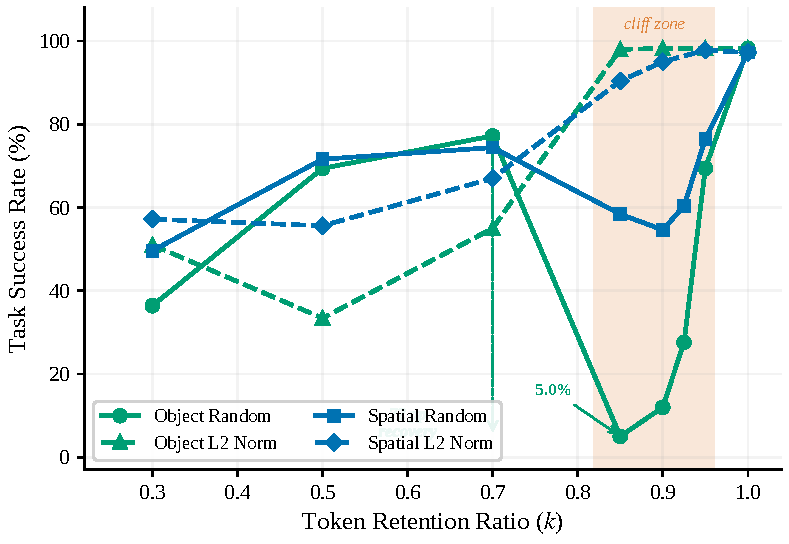
\includegraphics[width=0.85\linewidth]{figures/paper/fig_crosssuite.pdf}
\caption{$\pi_{0.5}$ cross-suite pruning profiles. Object random (green solid) exhibits a deep cliff at $k \in [0.85, 0.925]$ with 68\,pp recovery, absent on Spatial (blue solid). L2 norm (dashed) maintains a plateau on both suites through the cliff zone.}
\label{fig:crosssuite}
\end{figure}

The random cliff at $k \in [0.85, 0.925]$ is task-specific: Object collapses from 74.0\% ($k{=}0.95$) to 5.6\% ($k{=}0.85$), whereas Spatial retains 58.4\% at $k{=}0.85$ ($\Delta{=}53$\,pp between suites). Spatial random also exhibits mild non-monotonicity ($k{=}0.925$: 60.4\% $>$ $k{=}0.9$: 54.6\%, $\Delta{=}5.8$\,pp), but this is an order of magnitude smaller than Object's 68\,pp V-dip. The cliff pattern suggests Object manipulation concentrates critical information in specific token subsets whose removal is catastrophic at narrow retention bands; Spatial tasks distribute critical information more uniformly, tolerating moderate random removal without catastrophic failure.

L2 norm selection is consistent across suites at high retention ($k \geq 0.85$): Object and Spatial differ by $\leq 2.4$\,pp (Table~\ref{tab:pi05_crosssuite}). At $k \leq 0.7$, both suites exhibit the L2 V-shape (Object valley: 33.4\% at $k{=}0.5$; Spatial valley: 55.6\% at $k{=}0.5$), with Spatial maintaining higher absolute SR throughout. The method preference (random $>$ L2 at $k{=}0.5$; L2 $>$ random at $k{=}0.3$) is consistent across the two suites tested, suggesting the CV-strategy interaction may extend beyond a single task distribution.

\subsection{Token Importance Spatial Distribution}
\label{app:token_heatmap}

\begin{figure}[ht]
\centering
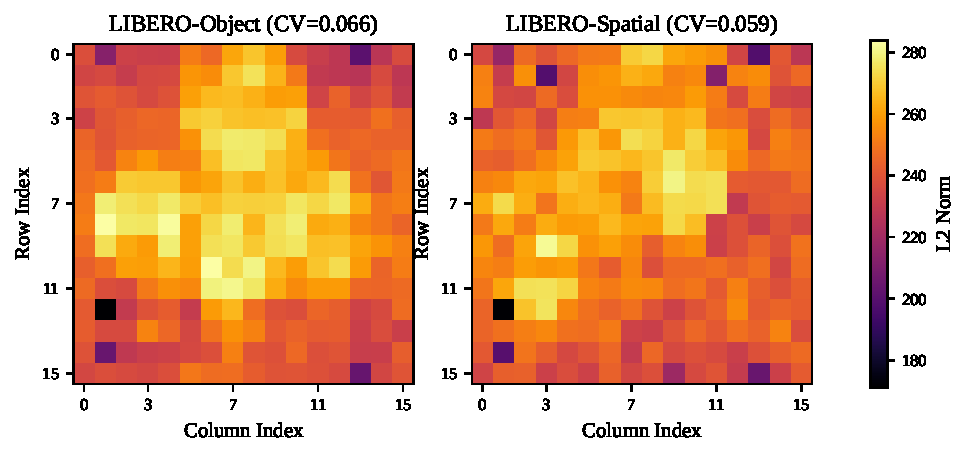
\includegraphics[width=0.85\linewidth]{figures/paper/fig_token_heatmap.pdf}
\caption{$\pi_{0.5}$ token importance spatial distribution (16$\times$16 grid, averaged over timesteps). Left: LIBERO-Object shows a pronounced center-high, edge-low pattern (center rows 7--9: norm $\sim$265--267; edge rows 0, 14--15: norm $\sim$235--236; CV${=}$0.066). Right: LIBERO-Spatial exhibits a flatter distribution (center-edge gap 14.67 vs.\ 21.87; CV${=}$0.059). The 33\% center-edge gap difference quantitatively explains Object's sharp cliff versus Spatial's graceful degradation under random removal.}
\label{fig:token_heatmap}
\end{figure}

Token importance heatmaps reveal that $\pi_{0.5}$'s 768 vision tokens (reshaped to a 16$\times$16 spatial grid after the $\sqrt{d}$-scaled linear projection) exhibit a center-high, edge-low L2 norm pattern. At $k{=}0.9$ (26 tokens removed), L2 norm-based selection discards predominantly edge tokens: 50\% of removed tokens fall in the outermost ring despite edge positions comprising only 23\% of the grid. This spatial concentration is consistent with the center tokens encoding the robot arm and target object, while edge tokens capture less task-relevant background.

Random removal at the same ratio samples deletions uniformly across the spatial grid, creating a combinatorial probability of simultaneously removing multiple high-importance center tokens. As more tokens are removed ($k{=}0.925 \to 0.85$), this probability increases sharply, consistent with the observed cliff onset. The asymmetry explains why L2 norm selection maintains a near-baseline plateau through the cliff zone: it preferentially preserves the high-importance center region that random removal disrupts by chance.

\subsection{Hypergeometric Cliff Model}
\label{app:cliff_model}

\begin{figure}[ht]
\centering
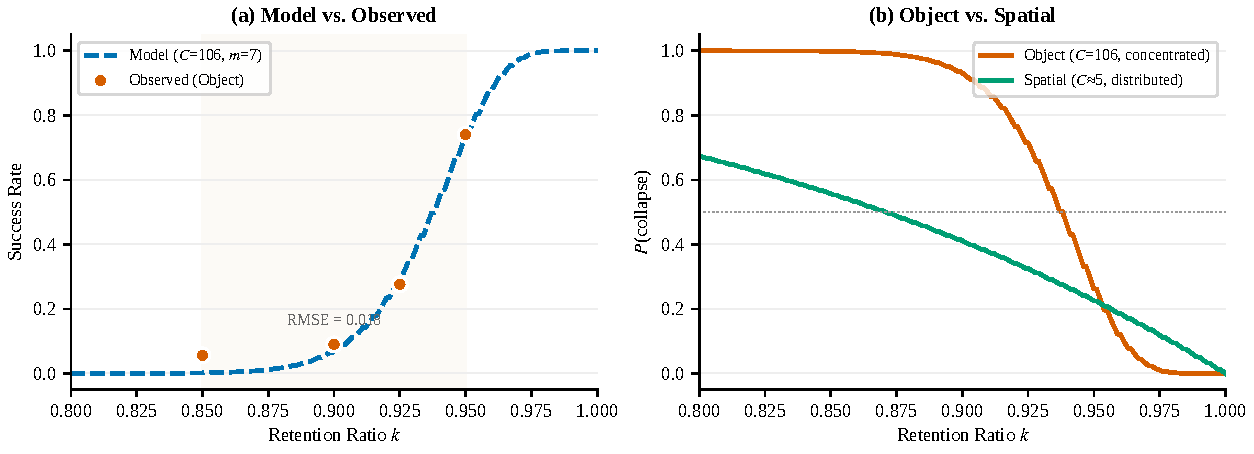
\includegraphics[width=0.85\linewidth]{figures/paper/fig_cliff_model.pdf}
\caption{Hypergeometric cliff model for $\pi_{0.5}$ Object random pruning. (a)~Model-predicted collapse probability (dashed) vs.\ observed success rate (solid) across the cliff zone $k \in [0.85, 0.95]$; RMSE${=}$0.018. (b)~$P(\text{collapse})$ curves for Object ($C{=}106$, concentrated) and Spatial ($C \approx 5$, distributed), illustrating why Object exhibits a sharp phase transition absent on Spatial.}
\label{fig:cliff_model}
\end{figure}

The random cliff on $\pi_{0.5}$ Object (Section~\ref{app:cross_suite_extended}) can be modeled as a hypergeometric sampling problem. Among $N{=}768$ vision tokens, $C{=}106$ are critical. $C$ and $T$ are jointly fit by minimizing RMSE against three cliff-zone data points ($k \in \{0.9, 0.925, 0.95\}$; all post-fix confirmed). When $\lfloor N(1{-}k) \rfloor$ tokens are removed uniformly at random, the number of critical tokens removed follows a hypergeometric distribution $\mathrm{Hypergeometric}(N, C, \lfloor N(1{-}k) \rfloor)$. We define performance collapse as removing $\geq T{=}7$ critical tokens simultaneously; the fit yields $C{=}106$, $T{=}7$ with RMSE${=}$0.018. The fitted $C{=}106$ (13.8\% of tokens) is broadly consistent with the top-importance center region identified in the token heatmap (Figure~\ref{fig:token_heatmap}), providing post-hoc interpretability: the ``critical tokens'' correspond to spatially concentrated, high-norm positions encoding the robot arm and target object.

The model predicts three characteristic retention ratios: $k{=}0.960$ where $P(\text{collapse}){=}10\%$ (cliff onset), $k{=}0.937$ where $P(\text{collapse}){=}50\%$ (midpoint), and $k{=}0.904$ where $P(\text{collapse}){=}90\%$ (near-complete collapse). The cliff width $\Delta k \approx 0.056$ between 10\% and 90\% collapse probability matches the observed transition from 74.0\% SR ($k{=}0.95$) to 9.0\% SR ($k{=}0.90$). At $k{=}0.85$ the model predicts near-certain collapse ($P{>}0.999$), consistent with the observed 5.6\% SR. The model captures the cliff onset and sharpness but does not explain the V-shape recovery at $k \leq 0.7$, where success rate rebounds to 74.0\%. The recovery lies outside the model's scope (which assumes monotonic collapse probability). We hypothesize that at aggressive pruning the model transitions to a qualitatively different computation regime, potentially relying on coarser spatial features that survive uniform subsampling, but this remains untested.

The cross-suite difference emerges naturally from the critical token count. Object manipulation concentrates critical information in $C{=}106$ tokens (13.8\% of the grid), creating a steep increase in $P(\text{collapse} \geq T)$ over a narrow $k$ range. Spatial tasks distribute critical information across approximately $C \approx 5$ tokens, making the probability of simultaneously removing $\geq T$ critical tokens negligible at all tested retention ratios, consistent with Spatial's graceful degradation (58.4\% at $k{=}0.85$ vs.\ Object's 5.6\%).

\subsection{OpenVLA Multi-Seed Consistency}
\label{app:openvla_multiseed}

\begin{table}[ht]
\centering
\small
\caption{OpenVLA success rates (\%) on LIBERO-Object under random token removal across two seeds (500 episodes each). All values are within 5\,pp, confirming the graded degradation curve is reproducible. Main text (Table~\ref{tab:main_results}) uses seed 42 for both L2 and random.}
\label{tab:openvla_multiseed}
\begin{tabular}{cccc}
\toprule
$k$ & Seed 7 (\%) & Seed 43 (\%) & $\Delta$ (pp) \\
\midrule
0.90 & 62.0 & 62.2 & $+$0.2 \\
0.70 & 49.0 & 44.4 & $-$4.6 \\
0.50 & 37.4 & 35.6 & $-$1.8 \\
\bottomrule
\end{tabular}
\end{table}

\subsection{L2 Norm vs.\ Random Scoring on OpenVLA}
\label{app:l2_vs_random}

\begin{table}[ht]
\centering
\small
\caption{OpenVLA cross-seed comparison on LIBERO-Object (500 episodes per configuration). L2 uses seed$\,{=}\,$42; random uses seed$\,{=}\,$7. Main text (Table~\ref{tab:main_results}) reports seed-42 random where available ($k{=}0.9$: 62.8\%, $k{=}0.5$: 35.8\%). Same-seed (seed42) random at $k{=}0.3$ yields 21.4\% (L2 outperforms by 3.6\,pp); same-seed at $k{=}0.7$ yields 44.4\% (L2 outperforms by 5.4\,pp). $\Delta$ is defined as L2$-$Random (positive indicates L2 advantage).}
\label{tab:openvla_l2_vs_random}
\begin{tabular}{cccc}
\toprule
$k$ & L2 Norm SR (\%) & Random SR (\%) & $\Delta$ (pp) \\
\midrule
0.95 & 70.6 & 69.4 & $+$1.2 \\
0.90 & 70.6 & 62.0 & $+$8.6 \\
0.70 & 49.8 & 49.0 & $+$0.8 \\
0.50 & 39.2 & 37.4 & $+$1.8 \\
0.30 & 25.0 & 20.6 & $+$4.4 \\
\bottomrule
\end{tabular}
\end{table}

\subsection{X-VLA Cliff Localization: Per-Task Analysis}
\label{app:xvla_cliff}

\begin{table}[ht]
\centering
\small
\caption{X-VLA per-task success rates (\%) at $k{=}0.80$ (40 of 50 tokens) and $k{=}0.85$ (42 of 50 tokens) on LIBERO-Object. Per-task breakdown is mean of 2 seeds (50 episodes per task per seed, 100 total); overall values are confirmed across 3 seeds ($89.0 \pm 0.7$\% at $k{=}0.80$, $67.9 \pm 0.3$\% at $k{=}0.85$). Despite retaining \emph{fewer} tokens, $k{=}0.80$ outperforms $k{=}0.85$ by 21.1\,pp overall. Four tasks (\textbf{bold}) suffer catastrophic interference ($\Delta \leq -50$\,pp) from two additional low-importance tokens (L2 rank 41--42 of 50) at $k{=}0.85$; the remaining six are unaffected ($|\Delta| \leq 10$\,pp). Cross-seed variance is $\leq 4$\,pp per task.}
\label{tab:xvla_cliff_pertask}
\begin{tabular}{lccr}
\toprule
Task & $k{=}0.80$ (\%) & $k{=}0.85$ (\%) & $\Delta$ (pp) \\
\midrule
alphabet\_soup & 100.0 & 100.0 & 0 \\
bbq\_sauce & 85.0 & 87.0 & $+$2 \\
\textbf{butter} & \textbf{57.0} & \textbf{0.0} & $\boldsymbol{-57}$ \\
\textbf{chocolate\_pudding} & \textbf{88.0} & \textbf{35.0} & $\boldsymbol{-53}$ \\
\textbf{cream\_cheese} & \textbf{98.0} & \textbf{45.0} & $\boldsymbol{-53}$ \\
\textbf{ketchup} & \textbf{79.0} & \textbf{27.0} & $\boldsymbol{-52}$ \\
milk & 85.0 & 95.0 & $+$10 \\
orange\_juice & 96.0 & 98.0 & $+$2 \\
salad\_dressing & 100.0 & 100.0 & 0 \\
tomato\_sauce & 98.0 & 91.0 & $-$7 \\
\midrule
\textbf{Overall} & \textbf{89.0} & \textbf{67.9} & $\boldsymbol{-21.1}$ \\
\bottomrule
\end{tabular}
\end{table}

The non-monotonic pattern is reproducible across both seeds: the same four tasks (butter, chocolate\_pudding, cream\_cheese, ketchup) exhibit catastrophic drops at $k{=}0.85$, while the remaining six maintain or improve performance. This task-specific sensitivity is consistent with the BART encoder creating entangled dependencies among marginal tokens: at $k{=}0.85$, two additional low-importance tokens (L2 rank 41--42) introduce interference that selectively disrupts tasks requiring fine-grained spatial discrimination. The four affected tasks all involve small, visually similar grocery items, while the robust tasks (alphabet\_soup, salad\_dressing) feature distinctive objects or high-contrast targets.

\subsection{VTR Per-Task Comparison}

\begin{table}[ht]
\centering
\small
\caption{VTR per-task success rates on LIBERO-Object for $M \in \{32, 64, 128\}$ (seed 42; 3-seed means are reported in Table~\ref{tab:vtr_results}). All three achieve similar overall SR (59.8\%--61.6\%), but individual task performance varies substantially across configurations, with per-task differences up to 30 percentage points.}
\label{tab:smart_compress_pertask}
\begin{tabular}{lcccc}
\toprule
Task & $M{=}32$ (\%) & $M{=}64$ (\%) & $M{=}128$ (\%) \\
\midrule
alphabet\_soup & 68 & 74 & 62 \\
bbq\_sauce & 46 & 56 & 34 \\
butter & 82 & 84 & 82 \\
chocolate\_pudding & 90 & 74 & 82 \\
cream\_cheese & 64 & 38 & 58 \\
ketchup & 66 & 64 & 62 \\
milk & 76 & 62 & 56 \\
orange\_juice & 28 & 46 & 58 \\
salad\_dressing & 60 & 64 & 54 \\
tomato\_sauce & 36 & 54 & 50 \\
\midrule
\textbf{Overall} & \textbf{61.6} & \textbf{61.6} & \textbf{59.8} \\
\bottomrule
\end{tabular}
\end{table}

\subsection{VTR Multi-Seed Results}

\begin{table}[ht]
\centering
\small
\caption{VTR success rates across three seeds on LIBERO-Object (500 episodes each). Mean $\pm$ std reported.}
\label{tab:multi_seed}
\begin{tabular}{lccccr}
\toprule
$M$ & Seed 42 & Seed 43 & Seed 44 & Mean $\pm$ Std \\
\midrule
32 & 61.6 & 59.2 & 59.6 & 60.1 $\pm$ 1.3 \\
64 & 61.6 & 60.0 & 64.4 & 62.0 $\pm$ 2.2 \\
96 & 52.6 & 58.2 & 52.8 & 54.5 $\pm$ 3.2 \\
128 & 59.8 & 54.0 & 60.2 & 58.0 $\pm$ 3.5 \\
\bottomrule
\end{tabular}
\end{table}


\section{VTR Full Results}
\label{app:vtr_full}

\begin{table}[ht]
\centering
\small
\caption{VTR re-encoding on SmolVLA (LIBERO-Object). Cross-attention and MLP adapter results report mean $\pm$ std over 3 seeds (500 episodes each). The M-curve is flat: $M{=}16$ (87.5\% compression) matches $M{=}128$ (passthrough) within 1.1\,pp. The baseline control (100K extra training, no compressor) confirms the gain is architectural. ``Compression'' = fraction of tokens removed.}
\label{tab:vtr_results}
\begin{tabular}{lccr}
\toprule
Configuration & $M$ & Compression & SR (\%) \\
\midrule
\textit{SmolVLA-Base (LoRA)} & 128 & 0\% & 44.8 \\
\textit{SmolVLA official} & 128 & 0\% & 59.2 \\
\textit{Baseline control (+100K steps)} & 128 & 0\% & 45.0 \\
\textit{Hard pruning (any $k$)} & -- & 5--50\% & 0.0 \\
\midrule
Cross-attn VTR & 16 & 87.5\% & 56.9 $\pm$ 1.3 \\
Cross-attn VTR & 32 & 75\% & 60.1 $\pm$ 1.3 \\
Cross-attn VTR & 64 & 50\% & \textbf{62.0 $\pm$ 2.2} \\
Cross-attn VTR & 96 & 25\% & 54.5 $\pm$ 3.2 \\
Cross-attn VTR & 128 & 0\% & 58.0 $\pm$ 3.5 \\
\midrule
MLP adapter ($\sim$22M) & 32 & 75\% & 63.4 $\pm$ 2.6 \\
\bottomrule
\end{tabular}
\end{table}


\section{Full VTR Ablation}
\label{app:smart_compress_full}

Table~\ref{tab:smart_compress_full} reports all five VTR configurations. The cross-attention module improves performance regardless of compression: $M \in \{32, 64, 128\}$ all achieve $\sim$60\% SR, exceeding the 44.8\% baseline by 15--17 points ($p < 0.001$, two-proportion $z$-test). Only at $M = 16$ (87.5\% compression) does performance decline modestly to 55.8\%, still 11 points above baseline. The $M{=}96$ dip (mean 54.5\% across three seeds, Table~\ref{tab:multi_seed}) may reflect an intermediate bottleneck that introduces representational redundancy without the regularization benefit of stronger compression ($M{=}32$, $M{=}64$).

Table~\ref{tab:cross_suite} reports performance across task suites. All suites are in-distribution: the training set (HuggingFaceVLA/libero) covers Object, Spatial, Goal, and Long. On LIBERO-Spatial, VTR achieves 53.2\% SR (vs.\ 0\% under hard pruning); on LIBERO-Goal, 56.4\% SR ($-6.6$pp from the 63.0\% unpruned baseline, vs.\ 0\% under pruning). The LIBERO-Goal decline indicates that re-encoding benefits vary across task structures even within the training distribution. Per-task results are in Table~\ref{tab:smart_compress_pertask}.

\begin{table}[ht]
\centering
\small
\caption{Full VTR ablation on LIBERO-Object across five compression levels. $M{=}32$ and $M{=}64$ achieve similar SR ($\sim$60\%); $M{=}96$ shows a modest dip; the $M{=}128$ passthrough confirms the gain originates from re-encoding.}
\label{tab:smart_compress_full}
\begin{tabular}{lcccrr}
\toprule
Method & $M$ & Reduction & SR (\%) & Episodes & Wilson 95\% CI \\
\midrule
\textit{Baseline} & 128 & 0\% & 44.8 & 500 & [40.5, 49.2] \\
\textit{Extended training} & -- & -- & 45.0 & 500 & [40.7, 49.3] \\
\textit{Hard pruning} & -- & 50--90\% & 0.0 & 500+ & [0, 0.76] \\
\midrule
VTR & 128 & 0\% & 58.0 & 1500 & $\pm$3.5 \\
VTR & 96 & 25\% & 52.6 & 500 & [48.2, 56.9] \\
VTR & 64 & 50\% & 61.6 & 500 & [57.3, 65.8] \\
VTR & 32 & 75\% & 61.6 & 500 & [57.3, 65.8] \\
VTR & 16 & 87.5\% & 55.8 & 500 & [51.4, 60.1] \\
\bottomrule
\end{tabular}

\vspace{2pt}
{\footnotesize $M{=}128$ reports mean $\pm$ std over 3 seeds (500 episodes each). Other VTR rows report single seed (seed 42) with Wilson 95\% CI. See Table~\ref{tab:multi_seed} for full multi-seed results.}
\end{table}


\section{VTR Evaluation Across Task Suites}
\label{app:cross_suite}

Table~\ref{tab:cross_suite} reports the performance of VTR ($M{=}32$) across three LIBERO suites. All suites are in-distribution: the training set (HuggingFaceVLA/libero) covers Object, Spatial, Goal, and Long (40 tasks, 1693 episodes total). On LIBERO-Goal, performance drops from 63.0\% to 56.4\% ($-6.6$pp). On LIBERO-Spatial, VTR achieves 53.2\% SR, where the official SmolVLA checkpoint scores 44.6\% and hard pruning yields near-zero (0.6\%). While 53.2\% nominally exceeds the official Spatial baseline, this difference concentrates in two of ten tasks (+44pp and +48pp respectively); the remaining eight tasks show a net difference of only +0.2pp. We therefore do not treat the Spatial comparison as evidence that re-encoding improves over the uncompressed official baseline. The qualitative pattern (cliff-edge vulnerability and re-encoding recovery) extends across the three tested task structures within the training distribution. The LIBERO-Goal decline indicates that re-encoding benefits vary across task structures.

\begin{table}[ht]
\centering
\small
\caption{VTR ($M{=}32$) evaluation across LIBERO task suites. All suites are in-distribution (training covers Object, Spatial, Goal, Long). Hard pruning (any method, $k{=}0.50$) produces 0\% or near-zero on all suites.}
\label{tab:cross_suite}
\begin{tabular}{lccc}
\toprule
Suite & Baseline (unpruned) & VTR $M{=}32$ & Hard Pruning $k{=}0.50$ \\
\midrule
Object & 44.8\% & 61.6\% & 0\% \\
Spatial & 51.8\% & 53.2\% & 0.6\% \\
Goal & 63.0\% & 56.4\% & 0\% \\
\bottomrule
\end{tabular}
\end{table}


\section{VTR Training Details}
\label{app:smart_compress_details}

The VTR module is a cross-attention pooling layer inserted between SmolVLA's pixel-shuffle vision connector and the SmolLM2 language backbone. It consists of $M$ learned query vectors that attend over the 128 vision tokens through standard multi-head cross-attention, producing $M$ compressed tokens as input to the LLM. The compressor adds 22.2M trainable parameters (approximately 5\% of SmolVLA's 450M total). Training is end-to-end: compressor and VLA policy parameters are jointly optimized.

\begin{table}[ht]
\centering
\small
\caption{VTR training hyperparameters. All configurations ($M \in \{16, 32, 64, 96, 128\}$) use identical procedures; only the number of query vectors differs.}
\label{tab:training_hyperparams}
\begin{tabular}{ll}
\toprule
Hyperparameter & Value \\
\midrule
\multicolumn{2}{l}{\textit{Model}} \\
\quad Base checkpoint & SmolVLA-Base (pretrained, before LIBERO fine-tuning) \\
\quad Compressor architecture & Cross-attention, 2 layers, 12 heads, dropout 0.1 \\
\quad Compressor parameters & 22.2M \\
\quad Total trainable parameters & 122.1M / 472.2M (25.85\%) \\
\midrule
\multicolumn{2}{l}{\textit{Optimization}} \\
\quad Optimizer & AdamW ($\beta_1{=}0.9$, $\beta_2{=}0.95$, weight decay $10^{-10}$) \\
\quad Learning rate & $10^{-4}$ \\
\quad Schedule & Linear warmup (1K steps, start factor 0.01) $\to$ cosine \\
\quad & annealing ($\eta_{\min}{=}2.5 \times 10^{-6}$) \\
\quad Max gradient norm & 10.0 \\
\quad Total training steps & 100,000 \\
\midrule
\multicolumn{2}{l}{\textit{Data \& batching}} \\
\quad Dataset & HuggingFaceVLA/libero (40 tasks, 1693 episodes across \\
\quad & Object, Spatial, Goal, Long suites) \\
\quad Batch size & 4 (no gradient accumulation)$^\dagger$ \\
\quad Num workers & 4 \\
\quad Eval interval & every 5K steps \\
\quad Checkpoint interval & every 1K steps \\
\midrule
\multicolumn{2}{l}{\textit{Hardware \& runtime}} \\
\quad Hardware & 1$\times$ NVIDIA RTX 4090 D (24GB) \\
\quad Precision & fp32 (no mixed precision) \\
\quad Wall clock & $\sim$6h 43m per configuration \\
\quad Training speed & 4.1 samples/sec \\
\quad Seed & 42 (seeds 43, 44 for multi-seed runs) \\
\midrule
\multicolumn{2}{l}{\textit{$M=32$ final metrics}} \\
\quad Train action loss & 0.11 \\
\quad Eval action loss & 0.052 \\
\midrule
\multicolumn{2}{l}{\textit{$M=64$ final metrics}} \\
\quad Train action loss & 0.045 \\
\quad Eval action loss & 0.062 \\
\bottomrule
\end{tabular}

\vspace{2pt}
{\footnotesize $^\dagger$The official SmolVLA checkpoint uses batch size 64 across 8 GPUs (effective batch size 512). Our batch size 4 on a single GPU contributes to the lower baseline SR (44.8\% vs.\ 87.3\%). All VTR configurations and the extended training control use this same batch size for fair comparison.}
\end{table}

The loss profile differs between configurations: $M=32$ has higher train loss (0.11 vs.\ 0.045) but lower eval loss (0.052 vs.\ 0.062), consistent with the smaller bottleneck acting as a stronger regularizer. Despite this loss difference, both achieve identical closed-loop success rates (61.6\%), reinforcing the finding that offline loss does not predict closed-loop performance (Section~\ref{sec:metric_disconnect}).

\subsection{MLP Adapter Control}
\label{app:mlp_adapter}

To verify that re-encoding effectiveness is not specific to cross-attention, we train a parameter-matched MLP adapter as a control. The adapter is a 3-layer feed-forward network with expansion ratio 4 (hidden dimension $4 \times d_{\text{model}}$), using average pooling for token reduction from 128 to $M$ tokens. Total parameters: 22.14M, matched to the cross-attention module's 22.2M. Training follows the identical protocol as VTR: SmolVLA-Base checkpoint, 100K steps, learning rate $10^{-4}$, batch size 4, same LIBERO dataset. At $M = 32$ (75\% reduction), the MLP adapter achieves $63.4 \pm 2.6$\% SR over 3 seeds, statistically indistinguishable from the cross-attention result ($60.1 \pm 1.3$\%; two-sample $t$-test, $p = 0.15$). This confirms that the re-encoding benefit does not depend on the specific module architecture.


\section{Offline Single-Step Action Error Analysis}
\label{app:offline_error}

Table~\ref{tab:offline_action_error} reports the single-step action prediction error under pruning, computed over 200 evaluation frames from LIBERO-Object. The unpruned model (bypass mode) produces actions with an L2 distance of 0.414 from ground truth; under learned-importance pruning at $k{=}0.50$, this increases to 1.391 ($3.4\times$). The per-dimension breakdown of the pruned-vs-unpruned difference reveals that the gripper dimension dominates (L2 = 1.02), corresponding to complete gripper state inversion on many frames. Position errors (0.20--0.30 per axis) are moderate individually but compound across the 7-dimensional action space. These single-step errors are large enough to push the robot off-trajectory within a few steps, explaining why 0\% of pruned episodes succeed in closed-loop evaluation despite moderate average offline metrics.

\begin{table}[ht]
\centering
\small
\caption{Single-step action prediction error (SmolVLA, $k{=}0.50$, learned scoring, zero-mask, 200 LIBERO-Object evaluation frames). Pruning increases action error by $3.4\times$ and introduces catastrophic gripper inversions.}
\label{tab:offline_action_error}
\begin{tabular}{lcc}
\toprule
Metric & Unpruned & Pruned ($k{=}0.50$) \\
\midrule
Action L2 vs.\ ground truth & 0.414 & 1.391 \\
Pruned vs.\ unpruned L2 & \multicolumn{2}{c}{1.284} \\
Relative action error & -- & 111.5\% \\
\midrule
\multicolumn{3}{l}{\textit{Per-dimension L2 (pruned vs.\ unpruned)}} \\
\quad Position $(x, y, z)$ & -- & 0.20, 0.25, 0.30 \\
\quad Rotation $(r_x, r_y, r_z)$ & -- & 0.01, 0.02, 0.01 \\
\quad Gripper & -- & 1.02 \\
\bottomrule
\end{tabular}
\end{table}


\section{Supplementary Figures}
\label{app:supplementary_figures}

% fig_pixel_shuffle moved to Section~\ref{sec:pixel_shuffle} in main text.

\begin{figure}[ht]
\centering
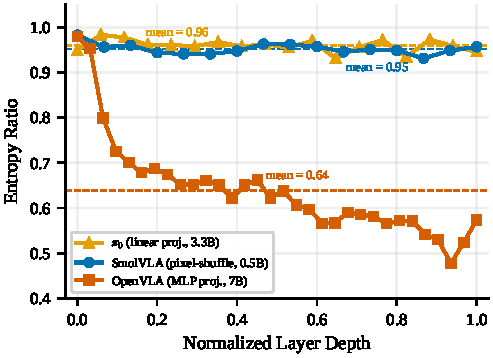
\includegraphics[width=\linewidth]{figures/paper/fig_entropy_layers.pdf}
\caption{Per-layer attention entropy ratio for SmolVLA (16 layers), OpenVLA (32 layers), and $\pi_{0}$ (18 layers). SmolVLA and $\pi_{0}$ maintain near-uniform attention throughout, while OpenVLA progressively sharpens from 0.98 to 0.48. Despite similar entropy, SmolVLA and $\pi_{0}$ exhibit opposite pruning outcomes due to token importance heterogeneity (CV $= 0.314$ vs.\ $0.038$). X-VLA (entropy $= 0.614$, CV $= 0.151$) occupies an intermediate position, consistent with its threshold-graded pattern (onset at $k{=}0.85$).}
\label{fig:entropy_layers}
\end{figure}


\section{Attention Entropy Measurement Details}
\label{app:entropy_details}

We measure the attention entropy ratio as the normalized Shannon entropy of the attention weights that the action decoder assigns to vision token positions. For a model with $N$ vision tokens, the entropy ratio is:
\begin{equation}
H_{\text{ratio}} = \frac{-\sum_{i=1}^{N} \alpha_i \log \alpha_i}{\log N}
\end{equation}
where $\alpha_i$ is the attention weight on the $i$-th vision token. The ratio ranges from 0 (all attention on one token) to 1 (uniform attention).

\paragraph{SmolVLA.} Measured on 2400 frames from LIBERO rollouts (overall entropy) and 260 frames across all 10 LIBERO-Object tasks (per-layer analysis across 16 layers). The mean per-layer entropy ratio is 0.95 (range: 0.93 to 0.98), consistent with near-uniform attention across all 128 vision tokens. The per-layer breakdown confirms this uniformity is not an averaging artifact:
\begin{itemize}[nosep]
    \item All 16 layers: 0.93--0.98 (spread 0.05)
    \item Minimum: layer 13 (0.93)
\end{itemize}
The flat profile across all processing depths confirms that pixel-shuffle tokens resist selective attention at every layer: because each token encodes 16 spatially contiguous patches via channel concatenation, all tokens are comparably information-dense, and the transformer has no basis for developing spatial selectivity.

\paragraph{$\pi_{0}$.} Measured on 100 frames from LIBERO-Object (tasks 20--29) across all 18 layers of the Gemma-based PaliGemma backbone (512 vision tokens: 256 per image $\times$ 2 cameras). The mean suffix-to-vision entropy ratio is 0.959 (range: 0.931--0.983, std 0.013), near-uniform across all layers with no progressive sharpening:
\begin{itemize}[nosep]
    \item All 18 layers: 0.931--0.983 (spread 0.052)
    \item Minimum: 0.931; Maximum: 0.983
\end{itemize}
The flat entropy profile, combined with $\pi_{0}$'s extremely low CV (0.038), is consistent with its high tolerance to pruning: tokens carry near-equal importance and receive near-equal attention. Removing any subset approximates uniform spatial downsampling, preserving a proportional share of the visual field without disrupting the attention distribution.

\paragraph{OpenVLA.} Measured on 250 frames from real LIBERO rollouts. The overall entropy ratio is 0.64. The layer-wise breakdown reveals progressive sharpening:
\begin{itemize}[nosep]
    \item Shallow layers (0--1): 0.95--0.98
    \item Early layers (2--4): 0.70--0.80
    \item Mid layers (12--20): 0.57--0.66
    \item Deep layers (24--30): 0.48--0.57 (minimum 0.48 at layer 29)
\end{itemize}
12.1\% of total attention weight falls on vision tokens overall, and within that fraction, the distribution is non-uniform in deeper layers. This progressive concentration indicates that OpenVLA has learned to selectively attend to task-relevant spatial locations, a pattern enabled by the MLP projector's preservation of per-patch spatial granularity.

\paragraph{Measurement conditions.} All models are measured on real LIBERO rollout data: SmolVLA on 2400 frames (overall entropy) and 260 frames (per-layer analysis), $\pi_{0}$ on 100 frames from LIBERO-Object, OpenVLA on 250 frames from 50 episodes $\times$ 5 initial frames. Sample size differences reflect computational constraints (OpenVLA's 7B forward pass is substantially more expensive), but all measurements use task-relevant visual inputs. Entropy statistics show low variance across frames (std $< 0.02$ for OpenVLA, std $= 0.013$ for $\pi_{0}$).


\section{Connector Architecture and Token Independence}
\label{app:connector_analysis}

The six-architecture taxonomy (Table~\ref{tab:model_properties}) spans a continuous spectrum of token independence structures, each associated with the vision-to-LLM connector rather than model scale or action head design.

Pixel-shuffle connectors create maximal entanglement. SmolVLA's $4 \times 4$ spatial folding packs 16 patches into each token by channel concatenation (CV $= 0.314$, the highest in our study). The folding is fixed and irreversible: removing one token eliminates an entire receptive field, and no downstream layer can recover the discarded content. Tokens encode non-overlapping spatial regions with heterogeneous visual content, making every token simultaneously essential and non-redundant.

Pure linear projections produce the opposite extreme. $\pi_{0}$ maps each SigLIP patch through a single linear layer with no cross-token interaction, yielding CV $= 0.038$ and near-maximal entropy (0.959). Tokens are genuinely interchangeable: any subset preserves the same per-patch information density as any other subset of equal size.

$\pi_{0.5}$ reveals a subtlety that $\pi_{0}$'s offline-only evaluation conceals. The $\times\!\sqrt{d}$ learned scaling preserves near-uniform norms (CV $= 0.055$), yet the closed-loop response is strongly method-dependent: random removal at $k{=}0.5$ retains 69.4\% SR while L2 norm-based removal collapses to 33.4\%. The 36\,pp gap arises because L2 ranking in a low-CV distribution selects spatially clustered tokens whose slight norm variations correlate with image regions, destroying the spatial coverage that this architecture requires. Token position analysis confirms this mechanism: at $k{=}0.5$, L2 selection produces a single dominant cluster containing 100\% of retained tokens with only 78\% spatial coverage, whereas $k{=}0.7$ yields two clusters with 97\% in the largest and 100\% coverage (Appendix~\ref{app:token_position}).

X-VLA's 12-layer BART encoder~\cite{lewis2020bart} introduces cross-token mixing through self-attention, creating partial dependencies that place it between the linear and MLP extremes (CV $= 0.151$, entropy $= 0.614$, the lowest among models). The resulting behavior is threshold-graded: performance holds through $k{=}0.9$ before a sharp cliff at $k{=}0.85$ ($-$31\,pp). The cliff onset is reproducible across three seeds (std $= 0.3$\,pp), confirming it as an architectural property.

MLP projectors (OpenVLA, OFT) apply per-patch non-linear transformations that create partial importance differentiation without cross-token entanglement. OpenVLA's CV (0.215) and OFT's CV (0.219) match within measurement noise, as do their entropy values (0.661 vs.\ 0.667); the connector, not the action head, is associated with token importance structure. CogACT~\cite{li2024cogact} corroborates the graded pattern from the literature (74.2\% SR under 78\% pruning).

Parameter count does not predict pruning tolerance. Ordered by scale: SmolVLA (450M) $<$ X-VLA (0.9B) $<$ $\pi_{0}$ (3.3B) $<$ $\pi_{0.5}$ (4B) $<$ OpenVLA (7B). Ordered by tolerance, SmolVLA remains the minimum, but $\pi_{0}$ and $\pi_{0.5}$ at 3.3--4B surpass OpenVLA at 7B, and X-VLA at 0.9B tolerates more aggressive pruning than OpenVLA. The CV spectrum (0.038 to 0.314) tracks connector complexity rather than parameter count across a 16$\times$ scale range.


\section{CV as Diagnostic Metric: Extended Analysis}
\label{app:cv_extended}
\label{sec:diagnostic}

Token importance CV correlates with both the tolerance class of a model and the optimal pruning strategy, a correlation that emerges from a single mechanistic principle: CV measures the strength of the importance gradient that scoring methods can exploit.

Low-CV models have near-uniform L2 norms. L2 norm ranking in this regime captures spatial artifacts (slight norm variations that correlate with image position) rather than genuine importance differences. Selection based on these artifacts concentrates retained tokens on spatially correlated patches, destroying the uniform coverage that low-CV architectures depend on. Random selection preserves spatial uniformity by construction. The mechanism predicts that the L2-over-random advantage should grow as CV increases, and the data in Table~\ref{tab:scaling_law} confirm this. On LIBERO-Object at $k{=}0.5$: $\Delta = -$36.0\,pp ($\pi_{0.5}$, CV $= 0.055$) $\to$ $-$26.9\,pp (X-VLA, CV $= 0.151$) $\to$ $+$3.4\,pp (OpenVLA, CV $= 0.215$). At $k{=}0.7$, the same ordering holds for $\pi_{0.5}$ and X-VLA ($-$22.2\,pp $\to$ $-$6.5\,pp); OpenVLA lacks a seed-matched pair at this ratio. The pattern persists across retention ratios, strengthening the interpretation from a coincidence at a single operating point to a structural property of the connector.

On simple manipulation tasks (Object), high-CV models present a genuine importance gradient where L2 norm ranking aligns with actual information content. OpenVLA (CV $= 0.215$) sits near the crossover on Object: L2 outperforms random by 7.8\,pp at $k{=}0.9$ where the gradient is most exploitable, shrinking to 3.4\,pp at $k{=}0.5$ as the proportion of removed tokens exceeds the gradient's discriminative range. On complex multi-step tasks, this advantage diminishes or reverses: OpenVLA Long at $k{=}0.9$ shows Random outperforming L2 by 3.2\,pp (46.8\% vs.\ 43.6\%), as compositional tasks distribute critical information across tokens with heterogeneous norm profiles (Section~\ref{sec:cv_sensitivity}).

Extreme compression introduces a partial reversal. At $k{=}0.3$, $\pi_{0.5}$'s L2 selection achieves $53.2 \pm 3.1$\% SR (2 seeds) vs.\ random's 36.4\%. When very few tokens remain, even spatially clustered high-norm tokens provide more signal than a sparse random sample. The V-shaped L2 curve is confirmed across seeds ($\sigma{=}0.1$\,pp at the $k{=}0.5$ valley). The reversal does not invalidate the CV diagnostic; it adds a budget-dependent interaction that future work should characterize across more models.

Attention entropy provides a mechanistic supplement that resolves an apparent paradox. SmolVLA's entropy (0.952) is nearly as high as $\pi_{0}$'s (0.959), yet SmolVLA collapses under any pruning. SmolVLA's tokens are uniformly \emph{attended} but carry heterogeneous \emph{content} due to pixel-shuffle folding. Entropy captures how the LLM allocates attention across tokens; CV captures the input-side importance structure. Entropy alone cannot distinguish ``interchangeable'' ($\pi_{0}$) from ``entangled'' (SmolVLA), but CV separates them cleanly (0.038 vs.\ 0.314). OpenVLA's progressive entropy sharpening from 0.98 to 0.48 across layers (Figure~\ref{fig:entropy_layers}) is consistent with a graded regime where the LLM progressively concentrates on higher-importance tokens.


\section{Why Re-Encoding Succeeds: Extended Analysis}
\label{app:reencoding_analysis}
\label{sec:learned_compression}

Learned re-encoding overcomes pixel-shuffle failure because it breaks the rigid spatial entanglement that the $4 \times 4$ folding creates. Cross-attention pooling integrates information across receptive field boundaries, redistributing content from the original 128 tokens into $M$ compressed representations no longer tied to fixed spatial blocks.

The $M{=}128$ passthrough configuration suggests that re-encoding, not compression, is the key factor. Passthrough adds parameters without reducing token count, yet gains 13\,pp over the baseline (44.8\% $\to$ 58.0\%). The relatively stable M-curve ($M{=}16$: 56.9\% closely matches $M{=}128$: 58.0\%, within 1.1\,pp) shows that once entanglement is broken, token count is secondary.

A parameter-matched MLP adapter (22.14M parameters) achieves 63.4\% SR at $M{=}32$, statistically indistinguishable from cross-attention ($p = 0.15$). Re-encoding through any learned mapping that integrates across token boundaries suffices; the attention mechanism itself is not essential.

The remedy is specific to the pathology. VTR succeeds precisely on architectures whose rigid spatial entanglement demands learned redistribution; for token-independent connectors where each patch already carries self-contained information, re-encoding is unnecessary.


\section{Offline Metrics Underestimate Closed-Loop Failure}
\label{app:offline_disconnect}
\label{sec:metric_disconnect}

Offline evaluation systematically underestimates pruning-induced failure because per-step averages dilute catastrophic single-step events that individually terminate episodes.

X-VLA at $k{=}0.3$ demonstrates the gap directly: offline loss is 1.0014 (near-baseline), yet closed-loop SR drops to $22.0 \pm 0.9$\% ($-$77\,pp). A single gripper inversion (L2 $= 1.02$) is a minor perturbation in average action error but terminates an episode irreversibly. $\pi_{0}$'s offline loss at $k{=}0.1$ shows a 2.4\% \emph{improvement} over the unpruned baseline (offline metrics only; no closed-loop evaluation available), a result that closed-loop evaluation may contradict if similar catastrophic events occur at deployment frequency.

$\pi_{0.5}$ adds a distinct form of evidence: the 36\,pp gap between L2 and random removal at $k{=}0.5$ is invisible to any offline metric that averages across token subsets or selection methods. Offline evaluation would report degradation for both methods; only closed-loop evaluation reveals that the \emph{choice} of pruning strategy, not just the pruning ratio, is associated with whether the model remains functional.


\section{Confounder Analysis}
\label{app:confounders}

The six architectures span three connector families but differ simultaneously in LLM backbone (PaliGemma for $\pi_{0}$/$\pi_{0.5}$, Llama-2 for OpenVLA, Florence-2 for X-VLA, SmolLM2 for SmolVLA), preventing clean isolation of the connector effect from backbone differences. The $\pi_{0}$--OpenVLA comparison (same 256 SigLIP-based tokens, different connector, backbone, and encoder fusion strategy) provides the closest available approximation, but a matched-backbone experiment remains the ideal control. This comparison involves differences in connector, backbone, and encoder fusion, limiting causal interpretation. Token count also varies across models (50 for X-VLA, 128 for SmolVLA, 256 for $\pi_{0}$/OpenVLA, 768 for $\pi_{0.5}$); the $\pi_{0}$--OpenVLA pair controls for this confounder within the CV analysis while still exhibiting the predicted CV-gap relationship.

The spatial clustering hypothesis for L2 failure on low-CV models is confirmed by token position analysis (Appendix~\ref{app:token_position}).

OpenVLA main-text results use seed 42 for both L2 and random. Cross-seed (seed 7) random comparison in Table~\ref{tab:openvla_l2_vs_random} confirms the L2 advantage is seed-independent: the gap ranges from $+$0.8 to $+$8.6\,pp across retention ratios regardless of random seed.


\section{Token Position Analysis}
\label{app:token_position}

To validate the spatial clustering hypothesis for L2 norm failure on low-CV models, we analyze the spatial distribution of tokens selected by L2 norm ranking on $\pi_{0.5}$ across three retention ratios.

At $k{=}0.7$ (538 of 768 tokens retained): DBSCAN clustering identifies 2 spatial clusters, with 97\% of retained tokens in the largest cluster and 100\% spatial coverage of the original image grid. The broad coverage explains why L2 selection still achieves 55.0\% SR at this retention ratio.

At $k{=}0.5$ (384 tokens retained): a single dominant cluster contains 100\% of retained tokens with only 78\% spatial coverage. The complete concentration into one spatial region confirms the clustering hypothesis: L2 norm ranking selects tokens from a contiguous high-norm region while abandoning 22\% of the spatial field. This is the retention ratio where L2 performance reaches its minimum (33.4\% SR, the V-shape valley).

At $k{=}0.3$ (230 tokens retained): 3 clusters emerge, with 86\% in the largest and 78\% spatial coverage. The fragmentation into multiple clusters at extreme compression is consistent with the partial L2 recovery observed at this ratio ($53.2 \pm 3.1$\% SR): when the budget is very small, L2 selection is forced to sample from multiple spatial regions, partially restoring coverage.

These results directly confirm that L2 norm ranking on low-CV models introduces spatial bias that degrades performance, and that the severity peaks at intermediate retention ratios where concentration is maximal.


\section{CV Scaling Law: Full Data}
\label{app:cv_scaling_table}

\begin{table}[ht]
\centering
\small
\caption{L2 norm vs.\ random removal at two retention ratios. The importance margin $\Delta$(L2$-$R) increases monotonically with CV at both $k{=}0.5$ and $k{=}0.7$: low-CV models require random selection (uniform importance $\rightarrow$ L2 degenerates to spatial clustering), while high-CV models tolerate either strategy on simple tasks (see Section~\ref{sec:cv_sensitivity} for task-dependent caveats). Data shown for LIBERO-Object; the monotonic ordering holds across retention ratios despite a 2$\times$ change in token budget.}
\label{tab:scaling_law}
\begin{tabular}{lccccc}
\toprule
Model & CV & Tokens & L2 SR (\%) & Random SR (\%) & $\Delta$(L2$-$R) \\
\midrule
\multicolumn{6}{l}{\textit{$k{=}0.5$ (50\% retention)}} \\
$\pi_{0.5}$ & 0.055 & 768 & 33.4 & \textbf{69.4} & $-$36.0 \\
X-VLA & 0.151 & 50 & 43.4$\pm$0.8 & \textbf{70.3}$\pm$0.9 & $-$26.9 \\
OpenVLA & 0.215 & 256 & \textbf{39.2} & 35.8 & $+$3.4 \\
\midrule
\multicolumn{6}{l}{\textit{$k{=}0.7$ (70\% retention)}} \\
$\pi_{0.5}$ & 0.055 & 768 & 55.0 & \textbf{74.0} & $-$19.0 \\
X-VLA & 0.151 & 50 & 58.6$\pm$0.4 & \textbf{65.1}$\pm$0.1 & $-$6.5 \\
OpenVLA\textsuperscript{$\dagger$} & 0.215 & 256 & -- & -- & -- \\
\bottomrule
\multicolumn{6}{l}{\footnotesize\textsuperscript{$\dagger$}$k{=}0.7$ omitted: no seed-matched L2/Random pair available.}
\end{tabular}
\end{table}


\section{CV-Strategy Interaction at Extreme Compression}
\label{app:cv_strategy_interaction}

The monotonic CV-gap relationship (Table~\ref{tab:scaling_law}) holds at $k{=}0.5$ and $k{=}0.7$, but partially reverses at $k{=}0.3$ for $\pi_{0.5}$. At this extreme budget, L2 norm selection achieves $53.2 \pm 3.1$\% SR (2 seeds) vs.\ random's 36.4\%, favoring L2 by $\sim$17\,pp. The reversal is consistent across both seeds (seed42: 51.0\%, seed43: 55.4\%; Table~\ref{tab:pi05_l2_multiseed}).

The mechanism is intuitive: when very few tokens remain ($k{=}0.3$ retains 230 of 768 tokens), even spatially clustered high-norm tokens provide more visual signal than a sparse random sample. At intermediate budgets ($k{=}0.5$, 384 tokens), random selection preserves enough spatial coverage to outperform L2's clustered selection; at extreme budgets, coverage from random selection becomes too sparse to be useful, and the concentrated signal from L2 selection dominates.

The interaction implies that the optimal pruning strategy depends on both CV and the absolute token budget. For low-CV models, the crossover point between random-preferred and L2-preferred regimes lies between $k{=}0.3$ and $k{=}0.5$. Characterizing this crossover across additional models and budgets is left to future work.


\section{Inference Cost-Benefit Analysis}
\label{app:cost_benefit}

The primary deployment benefit of VTR at this model scale is memory, not latency. Reducing from 128 to 32 vision tokens shrinks the KV-cache footprint for the vision portion by 75\%, a meaningful reduction for memory-constrained robotic hardware where KV-cache size can limit the number of concurrent policy instances or maximum context length.

End-to-end inference latency improves only modestly: 154.78\,ms at $M{=}32$ versus 164.33\,ms at full token count, a $1.06\times$ speedup (6\% reduction). At $M{=}64$: 156.16\,ms ($1.05\times$). The gap between token reduction and latency gain reflects SmolVLA's compact size (450M parameters): self-attention over 128 vision tokens is not the inference bottleneck, and the compressor's 22.2M-parameter cross-attention computation partially offsets downstream savings. Token pruning becomes a more compelling latency optimization for VLAs with larger token budgets ($>$256 tokens) or larger backbones (7B+ parameters), where attention cost scales quadratically with sequence length. Whether the training cost (100K steps, 6.5 hours per configuration) is justified depends on deployment context: for VLAs deployed across many tasks, the one-time training cost is amortized; for rapid prototyping, retraining is a barrier.

\paragraph{Comparison with the official checkpoint.}
VTR at $M = 32$ ($60.1 \pm 1.3$\% over 3 seeds) recovers from 0\% SR under hard pruning to performance comparable to the official SmolVLA checkpoint (59.2\%, CI [54.8\%, 63.4\%]). However, the difference is not statistically significant (two-sample $t$-test, $p \approx 0.72$), and the comparison should be interpreted cautiously given different training conditions (batch size 4 vs.\ 64, single vs.\ 8 GPUs). The primary contribution of VTR is recovering functional performance where all deletion methods yield 0\%, not matching the official baseline.

\subsection{Attention-Based Scoring Methods}
\label{app:attention_scoring}
\label{app:attention_pruning}

Attention-based scoring functions estimate token importance from the LLM's internal attention weights. Three principal variants exist: (i)~\emph{column-sum scoring} sums each vision token's received attention weight in the last transformer layer; (ii)~\emph{cross-layer mean scoring} averages column-sum scores across all layers; (iii)~\emph{attention rollout} multiplies attention matrices layer by layer (adding identity for residual connections) to approximate cumulative information flow. These methods require a full LLM forward pass and are backbone-specific. We focus on L2 and random in the main text because they operate solely on the connector output and suffice to reveal connector-dependent importance structure.

\subsection{Attention Entropy as Diagnostic}
\label{app:attention_entropy}

Attention entropy, defined as the mean Shannon entropy of the LLM's attention distribution over vision tokens, provides a complementary but less discriminative signal than CV. Three models with qualitatively different pruning behaviors cluster within a narrow entropy band: $\pi_{0.5}$ (0.666), X-VLA (0.614), and OpenVLA (0.661) span only 0.05 in entropy despite spanning 0.055 to 0.215 in CV. SmolVLA's entropy (0.952) is near-maximal, yet it is the least pruning-tolerant model. The discrepancy arises because entropy reflects the LLM's \emph{reading pattern} (how attention is distributed), while CV reflects the connector's \emph{writing pattern} (how information is distributed into tokens). The connector's output structure, not the downstream attention allocation, determines pruning robustness.

\subsection{Attention-Based Scoring Results}

Table~\ref{tab:attention_pruning} compares attention-based token scoring with L2 norm and random selection on X-VLA at $k{=}0.5$ (25 of 50 tokens retained). Three attention variants are evaluated: last-layer attention (attn\_last), mean attention across all decoder layers (attn\_mean), and attention rollout~\cite{abnar2020quantifying}.

\begin{table}[h]
\centering
\small
\caption{X-VLA success rates (\%) at $k{=}0.5$ across five scoring methods. Attention-based scoring recovers near-baseline performance across all suites while L2 norm falls below random on every suite. Bold indicates best per suite. \textsuperscript{*}Best of three attention variants.}
\label{tab:attention_pruning}
\begin{tabular}{lccccc}
\toprule
Suite & attn\_last & attn\_mean & attn\_rollout & L2 & Random \\
\midrule
Object & \textbf{99.2} & 98.4 & 97.4 & 43.4 & 70.6 \\
Spatial & 88.8 & 91.6 & \textbf{92.8} & 58.8 & 71.4 \\
Long & 90.2 & 94.0 & \textbf{94.8} & 45.0 & 61.6 \\
Goal & \textbf{98.2} & 97.4 & 96.8 & 59.0 & 67.2 \\
\bottomrule
\end{tabular}
\end{table}

L2 norm selection is anti-informative on X-VLA's entangling connector: L2 falls below random on all four suites, with gaps ranging from $-$8.2\,pp (Goal) to $-$27.2\,pp (Object). Attention-based scoring recovers near-baseline performance across all suites (${\geq}$92.8\%), with rollout peaking at 94.8\% on Long (seed43 confirms $\Delta{\leq}$0.6\,pp). On Object, all three attention variants achieve ${\geq}$97.4\%, far exceeding both L2 (43.4\%) and random (70.6\%). The mode ranking reverses across suites: last-layer attention is best on Object (99.2\%) but worst among attention methods on Spatial (88.8\%) and Long (90.2\%), while rollout shows the opposite pattern.

The L2 failure has a structural explanation. The BART encoder's 12-layer self-attention redistributes information across tokens, equalizing activation magnitudes (CV$\,{=}\,$0.151). L2 norms no longer reflect token importance; instead, they select spatially correlated clusters that miss critical information. Goal L2 exhibits non-monotonic behavior ($k{=}0.7$: 53.4\% $<$ $k{=}0.5$: 59.0\%), confirming that retaining more L2-selected tokens is actively harmful. Per-task variance under L2 pruning is extreme on Spatial (std$\,{=}\,$31.5\,pp, range 0--92\%), while attention scoring keeps all tasks above 80\%. The double dissociation extends to $\pi_{0.5}$, where attention scoring at $k{=}0.5$ exhibits suite-dependent failure (Table~\ref{tab:pi05_attention_crosssuite}). On three suites (Goal, Spatial, Long), attention performs within noise of random ($\pm$3\,pp). On Object, attention collapses to 37.8\% ($-$31.6\,pp vs.\ random's 69.4\%), a catastrophic failure unique to tasks requiring spatial discrimination among visually similar alternatives. The linear connector produces an extremely narrow attention score range ($[2{\times}10^{-6},\, 3.6{\times}10^{-3}]$) with systematic position bias favoring early tokens; on Object, this bias selects semantically relevant but spatially uninformative tokens, destroying the fine-grained spatial information needed for target identification.

\begin{table}[ht]
\centering
\small
\caption{$\pi_{0.5}$ attention vs.\ random at $k{=}0.5$ across LIBERO suites. Attention is neutral on 3/4 suites but catastrophically harmful on Object.}
\label{tab:pi05_attention_crosssuite}
\begin{tabular}{lccc}
\toprule
Suite & Attention (\%) & Random (\%) & $\Delta$ (pp) \\
\midrule
Goal & 71.2 & 73.6 & $-$2.4 \\
Spatial & 72.6 & 71.6 & $+$1.0 \\
Long & 49.4 & 46.8 & $+$2.6 \\
Object & 37.8 & 69.4 & $-$31.6 \\
\bottomrule
\end{tabular}
\end{table} By contrast, $\pi_{0.5}$'s L2 norms do reflect importance: on Goal, L2 outperforms random by $+$35.2\,pp at $k{=}0.85$, decaying to $+$5.4\,pp at $k{=}0.95$ (log-decay trend across four retention ratios). This yields a connector-dependent scoring reversal: attention is effective on entangling connectors but not token-independent ones, while L2 norm shows the converse (Figure~\ref{fig:scoring_crossover}).

\begin{table}[h]
\centering
\small
\caption{Scoring reversal summary: $\Delta$ vs.\ random at $k{=}0.5$, except \textsuperscript{*}Goal suite across $k \in [0.85, 0.95]$. Compact view of the pattern shown in Figure~\ref{fig:scoring_crossover}.}
\label{tab:scoring_crossover_summary}
\begin{tabular}{lcc}
\toprule
& Attention & L2 norm \\
\midrule
Entangling (X-VLA) & Effective ($+$31\,pp) & Anti-inform.\ ($-$8 to $-$27\,pp) \\
Token-indep.\ ($\pi_{0.5}$) & Ineffective\textsuperscript{$\dagger$} ($-$2 to $-$32\,pp) & Effective\textsuperscript{*} ($+$35.2$\to$$+$5.4\,pp) \\
\bottomrule
\multicolumn{3}{l}{\footnotesize\textsuperscript{$\dagger$}Neutral on 3/4 suites ($\pm$3\,pp); harmful on Object ($-$31.6\,pp).}
\end{tabular}
\end{table}


\section{AI Disclosure}
\label{app:ai_disclosure}

AI tools assisted code development and manuscript drafting; all scientific claims, experimental designs, and interpretations are the authors' own.